\documentclass[journal,twocolumn,12pt]{ieeesyscoin}
\usepackage{cite}
\usepackage{amsmath,amssymb,amsfonts}
\usepackage{algorithmic}
\usepackage{enumitem}
\usepackage{caption}
\usepackage{xcolor}
\usepackage{graphicx}
\usepackage{textcomp}
\usepackage{multirow}
\usepackage{lipsum}
\usepackage{makecell}
\usepackage[switch]{lineno}
\def\BibTeX{{\rm B\kern-.05em{\sc i\kern-.025em b}\kern-.08em
    T\kern-.1667em\lower.7ex\hbox{E}\kern-.125emX}}
\begin{document}

\history{}

\title{\centering DAOSYS: Smart DAO Protocol for Decentralized Finance}
\author{\centering  \uppercase{Cyotee Doge}\authorrefmark{1}, 
\uppercase{Ian C. Moore, PhD}\authorrefmark{2},
\uppercase{Ryland Arbour}\authorrefmark{3}, and
\uppercase{Jagdeep Sidhu, MSc}\authorrefmark{4}}

\address[1]{\centering DAO Advisor, Syscoin Platform (e-mail: cyotee@syscoin.org)}
\address[2]{\centering  Syscoin Researcher, Syscoin Platform (e-mail: imoore@syscoin.org)}
\address[3]{\centering  L2 Advisor, Syscoin Platform (e-mail: rylandarbour@syscoin.com)}
\address[4]{\centering Syscoin Lead Developer, (e-mail: sidhujag@syscoin.org)}
\tfootnote{}

\markboth
{Cyotee \headeretal: DAOSYS: Smart DAO Protocol for Decentralized Finance}
{Cyotee \headeretal: DAOSYS: Smart DAO Protocol for Decentralized Finance}

\corresp{}

\begin{abstract}
Despite popular perception, treasuries of Decentralized Autonomous Organizations (DAOs) tend to be centrally controlled and do not reflect the true ethos of cryptocurrency (i.e., \textit{not your keys, not your coins}). DAOSYS solves this problem with its new Autonomous Service Engine (ASE) technology by deploying a reference platform for self-sovereign capital coordination. Through the ASE, the DAOSYS token will serve as a protocol layer creating a fully backed non-speculative asset allowing for quick seamless deployment of child DAOs in a secure manner. This is made possible by innovating on the multi-faceted proxy standard defined in EIP-2535. The ASE will serve as the cornerstone of all SYS Labs decentralized finance (DeFi) products, as supported by the Syscoin Platform.
\end{abstract}

\begin{keywords}
DAOSYS, Smart DAO, Decentralized Finance, Hyper-diamond proxy, EIP-2535
\end{keywords}

\titlepgskip=-15pt

\maketitle

\section{Introduction}
\label{sec:introduction}

The objective of a decentralized autonomous organization (DAO) is to solve the principal-agent dilemma. This dilemma is a result of misaligned incentives where agents acting in a system are incentivized towards their own benefit over the benefit of a principle or other agents acting within the system \cite{San83}. Typically, these are found in centralized systems where the central acting authority is the main compromised agent. The DAO solves this by decentralizing the governance process through the utilizing of smart contracts running on open source blockchains.

The first inception of the DAO concept happened in May 2016 out of the Ethereum community, which was known as Genesis DAO, and was built as a smart contract on the Ethereum blockchain. However, this resulted in the well known DAO Hack which resulted in the draining of \$60M USD worth of funds from its treasury \cite{Sie22}. Today, there are many DAOs in operation with Uniswap, Aave and Maker DAO being amongst the most popular. However, these DAOs still fundamentally violate the core value proposition of self sovereignty that crypto currency promises, where DAOs currently take ownership of capital managed in a treasury controlled by a few individuals. This is the problem that DAOSYS intends to address.

DAOSYS vision is to operate like a pure automated market maker (AMM) and be implemented in a manner that does not require external controls. In 2018, Uniswap became the first decentralized platform to successfully utilize an AMM \cite{Uni19}. However, like Uniswap and many AMMs, control of the capital in their respective liquidity pools is still centralized. DAOSYS intends to address this core issue via its new Autonomous Service Engine (ASE) technology \cite{Sys22}, hence allowing DAOs to be more autonomous and fully decentralized. The DAOSYS token is a smart DAO protocol is that fully backed by an index of assets supported by its child DAOs. This technology will allow users to test, implement and realize countless decentralized finance (DeFi) usecase designs deployed in a secure manner through the ASE without having to continually redeploy new builds.

\begin{figure}[h!]
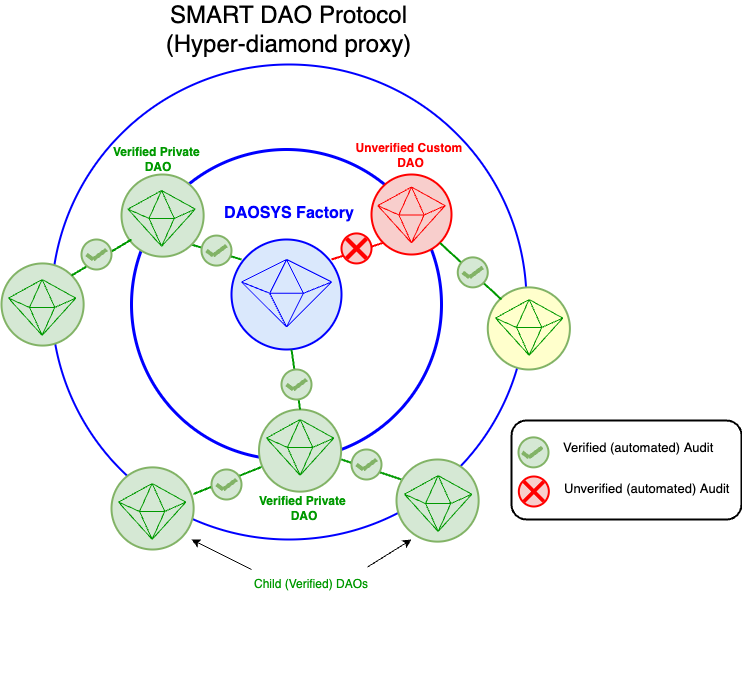
\includegraphics[width=3in]{img/smart_dao.png}
\caption{DAOSYS as the smart DAO protocol, utilizing the hyper-diamond proxy; see EIP-2535 in Appendix A} 
\label{fig:daosys_governance}
\end{figure}

The features that DAOSYS will have are as follows:

\begin{itemize}
  \item Smart DAO protocol via hyper-diamond proxy
  \item Self-sovereign via trustless automatic integration
  \item Seamless fast deployment using secure templates
  \item Hyper-diamond standard
  \item Collateralized VE (vesting) indexing token
  \item Automated audits of child DAOs
  \item Fully backed (eg, DAI, SYS)
  \item Non-speculative asset
  \item No code or low code deployments via user interface
  \item New emergent behavior and innovation for DeFi
\end{itemize}  

\section{Governance}
\label{sec:governance}

DAOs are governance structures for groups of people to come together and make decisions, which is one of its main distinguishing features. Unlike traditional organizations (e.g., private companies, non-governmental organizations, charities, etc.) which have a centralized structure, these decisions are coordinated and enforced on a blockchain in a decentralized manner. Since DAOSYS proposes to be autonomous and fully decentralized, it has no top level governance.

AMMs are an essential part of the DeFi ecosystem. They allow digital assets to be traded in a permissionless and automatic way by using liquidity pools rather than a traditional market of buyers and sellers. Applying the AMM model to DAOs means that users create their own treasuries for specific ventures. These treasuries may apply a variety of governance solutions along with their treasuries. This allows for a compartmentalization of the politics that arise with any governance solution from the actual treasury management.

Under this model, the Syscoin Foundation behaves more like the software vendor. The factory makes open-source reference implementations of DeFi components available to compose into treasuries. Updates to these smart-contracts are available for deploying new pools that may be added to a DAO. Hence, this removes the need for top-level governance solutions that decides whether to include an update because users are free to create new pools.

A user creates a DAO by selecting which vaults and bond markets they would like to include. These vaults may come from one of four sources.

\subsection{Reuse an existing vault}

This works best for when users wish to maintain their position in one DAO, but want to add more pools to form a new DAO.

\subsection{Recreate an existing vault}

As the adage goes, \textit{if it’s not broke, don’t fix it}. The investment strategy implemented in a vault can be used across several instances of vault pools. This works well for new DAOs that wish to replicate the financial strategies of an existing DAO. Also, this also works for when a new DAO would like to invest in other DAOs using the same strategy.

\subsection{New pool with new investment strategy}

A user may wish to create a new DAO reusing functionality available from the factory, but configured in a novel manner. The flexibility available in the ASE means that even a simple strategy has several configuration options. This is useful for when a DAO wishes to adopt a novel investment strategy that might not have been previously viable.

\subsection{New pool with custom code}

The Syscoin Foundation makes internal decisions regarding what smart-contracts are available through the factory similar to open source software development. Because this only concerns the software available from the foundation, this does not need to be open to public governance. When the community at large wishes to release custom code outside the foundation, a user may use the factory to deploy their own factory offering their custom code. This new factory inherits the offerings of the parent factory and may add their own modules.

These pools form the foundation of the DAO. Autonomous and permissionless liquidity pools that act as the agreed upon foundation for DAO treasury management. From there users may launch further liquidity pools that may accept the DAO's Treasury Token for deposit. These form the Roundtables for managing ventures within the DAO. The Roundtables compartmentalize management teams, Councillors, of the various ventures being executed under a DAO’s mission statement. A Roundtable typically does not have it’s own governance token, instead using a Council Token to resolve disputes by executing buyout options.

From the Roundtables, any Councillor may use their contribution to the Roundtable to launch a bond offering for a Quest. Quests define the bounty award and terms for completing a task. The Councillor that issues the Quest puts their share of the treasury in escrow to fund it. The interest being earned from that underlying position is then split to fund the bounty, compound into that position, and to sell on the bond market. This ensures that Questors know the payment for work they deliver is secured. And protects the Councilor from failure to deliver; see Fig. \ref{fig:daosys_governance} for outline.

\begin{figure}[h!]
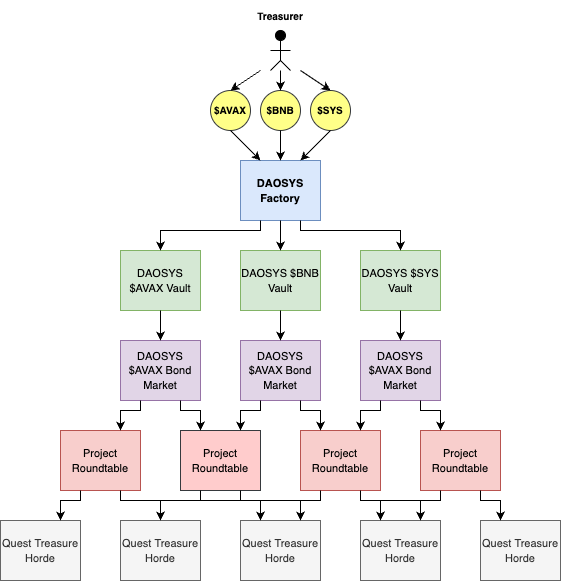
\includegraphics[width=3in]{img/governance.png}
\caption{DAOSYS Governance Structure: new pool with custom code (ie, Quests)} 
\label{fig:daosys_governance}
\end{figure} 

\section{Architecture}
\label{sec:architecture}

The innovative software architecture that allows DAOSYS to pioneer a revolution in DAOs is the ASE. This introduces a revolution allowing DAOs to become more autonomous and fully decentralized. The ASE iterates on the Diamond proxy standard from EIP-2535 (see Appendix \ref{sec:diamond}) to apply AMM functionality for more flexible capabilities.

\subsection{ICreate2Metadata}

The \texttt{CREATE2} opcode is a low level human readable instruction used within the stack-based architecture of the Ethereum Virtual Machine (EVM) that was introduced in 2019 with EIP-1014 \cite{But18}. This is the technology that enables AMMs in EVM implementations which allows a smart-contract to deploy another smart contract, and is typically called the Factory design pattern. Protocols like Balancer and Uniswap provide the ability to create permissionless liquidity pools. However, the limit of these implementations is the immutable nature of smart-contract bytecode as they can only deploy a single type of contract. 

All contracts deployed through the ASE, new service proxies and delegate service, store the metadata for their deployment. This includes the factory address they were deployed from, and the value used to salt their deployment. Combined with the contract’s \texttt{codehash} this can be used to recalculate the contract’s address from the assertion of it’s \texttt{ICreate2Metadata} interface hook.

\subsection{IDelegateService}

Protocols like Aavegotchi have pioneered smart-contract architecture by iterating on the proxy capabilities of the EVM to advance the Factory design pattern. Smart-contract proxies take advantage of the \texttt{DELEGATECALL} opcode to allow a smart-contract to reuse the logic implemented in other smart-contracts. The Autonomous Service Engine advances this innovation with an infinitely flexible Diamond Factory design. The Diamond Factory design factory combines the Factory and Diamond design patterns to deploy configurable proxies. This allows for infinitely composable proxies.

Delegate Services replace the Facets defined in ERC-2535; see Fig. \ref{fig:hyper_facet}. Delegate Services define a strict storage allocation and access standard beyond the theory presented in ERC-2535. A Service is a smart-contract or library implemented following the Deterministically Dynamic Storage Allocation standard. A Service also reports the factory that deployed that contract and the salt used during deployment. This way the recalculation of the address from the factory init code hash and salt can be used to verify new Services as an implicit ACL.

This means that the deployment process for new Services deviates from industry standard. New Services are deployed as compiled bytecode passed to the Service Proxy Factory as the argument for the deployment function. The Service Proxy Factory then instantiates that bytecode as a new contract. ASE compliant Services must include the \texttt{ASEServiceBootstrapper} library to retrieve the address salt to initialize the Service. This should be done by delegating to the canonical external library deployment. ASE compliant external libraries may precalculate their address salt and store it as a constant. The standard Service initialization functions must still be implemented, but may hard code the values and return values since they can not store state.

All Services are required to implement ERC-165 including the Service extension that enumerates the functions. The Service extension to ERC-165 includes a per interface enumeration of the function selectors that define the interface ID. Additionally, there is an enumeration of all the function selectors across all interface IDs, and a \textit{ServiceDef} struct that includes the information for initializing a Service Proxy to consume the Service.

\begin{figure}[h!]
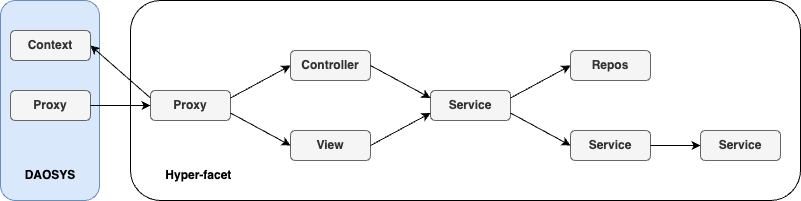
\includegraphics[width=3in]{img/hyper_facet.png}
\caption{Hyper-facet consisting of delegate Services that replace facets defined in ERC-2535} 
\label{fig:hyper_facet}
\end{figure} 

\section{Security}
\label{sec:security}

When a DAO joins the DAOSYS ecosystem it will be either verified or unverified, which is a security attribute that will dictate the way it conducts itself on the network. This verification is done automatically and trustlessly based on the configurations it adopts upon launch. Within that classification, it will be further subclassed as either private or public. Hence, the four types of security are: public verified, private verified, public unverified, and private unverified.

\subsection{Verified DAOs}
\label{sec:verified}

The main purpose of verified DAOs is to ensure that contributing DAOs are safe to transact with from a security standpoint, as DAOSYS will know what contracts will be doing with storage and will be participating in the tokenomics model described in Section \ref{sec:tokenomics}. The public verified usecase will be the most common type of DAO on the network and are essentially clones of DAOSYS. With this comes the ability to create is own sub-network of child DAOs where it will receive the benefit of cascading royalties as illustrated in Fig. \ref{fig:clone_model}. The freedoms on launching a public verified DAO would akin to the GNU public licence in the sense that there would be certain freedoms that users would be permitted and not permitted to do with the source code.

A private verified DAO would be the second most adopted usecase on the network having freedoms akin to a Redhat or AWS EC2 licence agreement where participation in the DAO is free, but services and support are not. A likely scenario of this would be corporations looking to set up private smart wallets to consume the DAOSYS features.

\subsection{Unverified DAOs}
\label{sec:unverified}

When a newly launched DAO contains facets augmented to configurations that do not adhere to the DAOSYS standards, then it is classified as unverified. For users that are not proficient in Solidity development and security then there is an increased risk that users of unverified DAOs could loose their funds. However, that does not mean that there are not good usecases for these types of DAOs. For instance, a public unverified DAO may be used as a public testnet to vet new ideas that are uncommon to the network. Whereas a private unverified DAO may be useful to those looking setup smart wallets with modules consisting of a host of sophisticated asset managing DeFi strategies. These modules will allow users to configure their own DeFi strategies and would be akin to players in traditional finance setting up their own LLCs to manage funds.

\section{Tokenomics}
\label{sec:tokenomics}

The tokenomics model representing the minimum commitment of verified child DAOs is illustrated in five steps in Fig. \ref{fig:tokenomics_model}. This model represents a symbiotic relationship between DAOSYS and its respective child DAOs. This is where verified child DAOs receives the interest generated from its own collateral and DAOSYS receives debt-based interest generated from that collateral.

Included in this symbiotic relationship are several other benefits that child DAOs will have by joining this network over building its own standalone DAO. New DAOs benefit from significantly fast development time by selecting any one of the pre-vetted, secure DAOSYS templates. Included in this, DAOs can simulate the tokenomic behavior prior to launch using our Python simulator tailored to our system (as detailed in Section \ref{sec:python_simulator}) to build predictive models to determine future estimated ROI calculations. DAOs that are part of our network will also benefit from the seamless integrations of working with other participating DAOs. These integrations would be akin to the benefits nation states have when they join international trade agreements, where DAOSYS behaves as the overseeing regulatory body, and the child DAOs share attributes as participating nation states. These child DAOs also have the flexibility of cloning the DAOSYS factory and spawning its own sub-network within the DAOSYS ecosystem; see Fig. \ref{fig:clone_model}.  

\subsection{Tokenomics Model}
\label{sec:tokenomics_model}

The five steps of the tokenomics model described in Fig. \ref{fig:tokenomics_model} are as follows. In step A we initially assume DAOSYS vaults contains no assets, while the child DAO vaults have 1000 SYS and 200 DAI. In step B we have a triggering event that stimulates a small deposit of 1 SYS and 0.2 DAI from the Child DAO vaults into the DAOSYS vaults. When this happens the DAOSYS vault will mint debt tokens of these newly acquired assets with a 1:1 backing. In exchange for these assets, the child DAO will receive newly minted index tokens that represent a 1:1 backing by DAOSYS. Next in step C, DAOSYS will send both these debt and collateral tokens through a DeFi investment engine. Over time, the DAOSYS vault will collect interest from these newly acquired collateral and debt assets, as seen in step D. The child DAO can either keep these collateral in DAOSYS and continue to collect interest or recall the collateral. Hence, finally in step E of this process, the child DAO recalls the original collateral and all its earned interest, while DAOSYS keeps the debt interest. Once the child DAOs collateral and interest is withdrawn, both dept and index tokens are burned. When comparing the final step to the initial step, we see that both DAOSYS and the child DAO see a net positive gain in liquidity. The child DAO will collect interest from its own collateral, while DAOSYS will collect interest from the debt created from that collateral. 

\begin{figure}[h!]
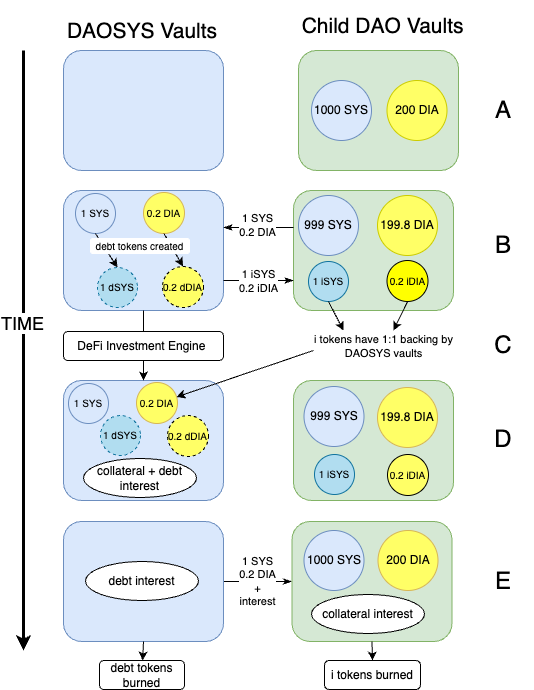
\includegraphics[width=3in]{img/tokenomics_model.png}
\caption{Tokenomics model representing minimum commitment of publicly and privately verified child DAOs} 
\label{fig:tokenomics_model}
\end{figure} 

\subsection{Clone Model}
\label{sec:clone_model}

When considering the outline of Section \ref{sec:tokenomics_model}, we can see emergent behaviour that will arise for DAOs that are also clones of DAOSYS as illustrated in Fig. \ref{fig:clone_model}. When considering the tokenomics model in Section 
\ref{sec:tokenomics_model}, there will arise a bidirectional cascade effect where DAOSYS will receive the cascaded interest accumulated on debt, and the the child DAOs will receive the cascaded interest accumulated on collateral.

\begin{figure}[h!]
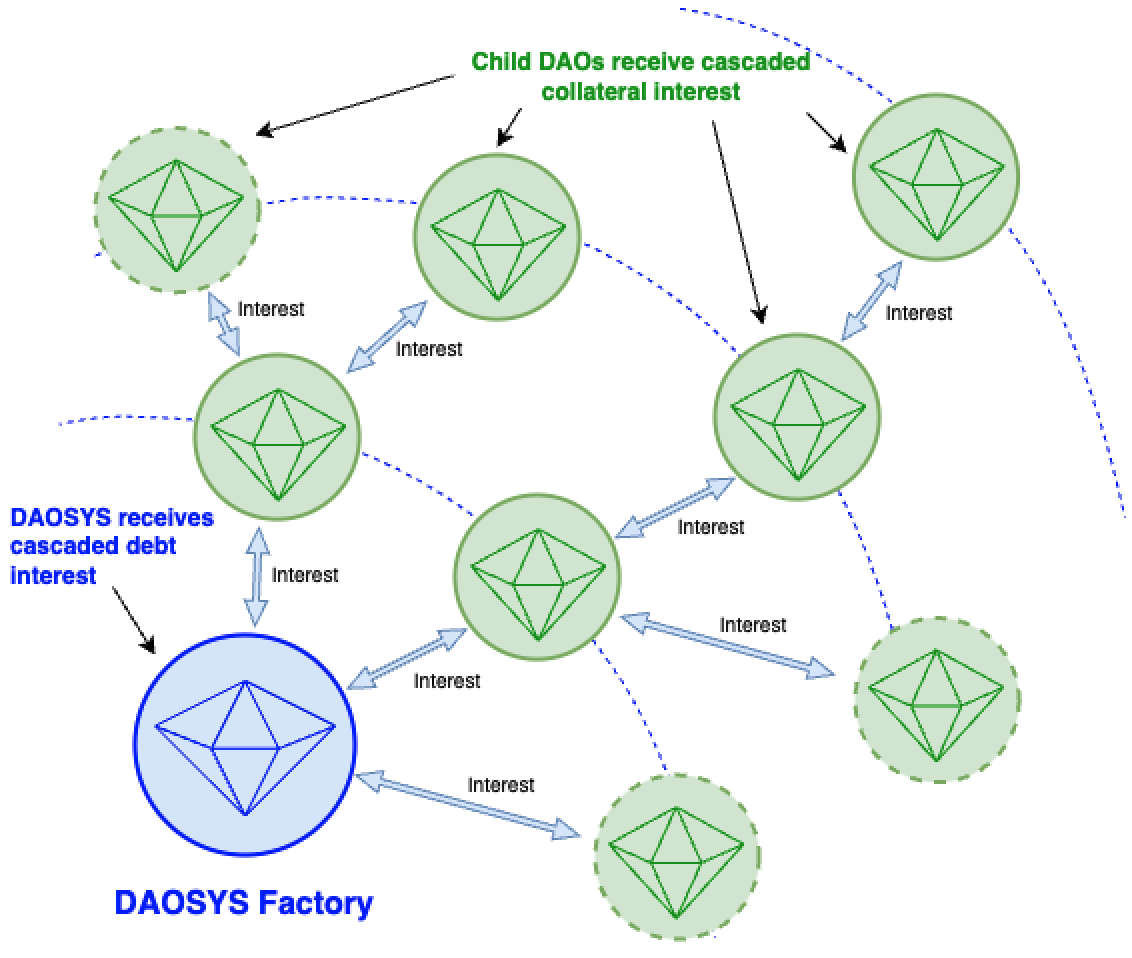
\includegraphics[width=3in]{img/clone_model.png}
\caption{Clone model that emerges from the tokenomics model of Fig. \ref{fig:tokenomics_model} which occurs as a byproduct from child DAOs creating their own children; collateral interest generated by DAOSYS cascades up through inheritance structure to all respective verified child DAOs, while debt interest cascades down to DAOSYS} 
\label{fig:clone_model}
\end{figure} 

\subsection{DeFi Python Simulator}
\label{sec:python_simulator}

To realize proper tokenomics design, it is highly inefficient to invest resources into development without first conducting a proper simulations of the design to test specifications for various outcomes. This is what every DeFi project in the crypto space is not doing. This is why we are introducing an open source python package to simulate various sandboxed DeFi components of DAOSYS so that project engineers, managers and designers can pre-plan outcomes prior to investing valuable resources into development.

With this tool, DAOSYS designers can utilize the plug and play components of our simulator to build tokenomics mockups for business planning purposes so that teams can come together and get collective consensus alongside potential users and investors. Not only is this tool applicable to DAOSYS, it can be used as a general purpose tool to simulate DEX activity for anyone wishing to setup their own liquidity pool (LP) and wish to stress test their ideas prior to development. This can be used as a powerful design tool to explore the limitations of an DeFi project idea prior to committing valuable resources on development costs (ie, Devs and Project Managers). Table \ref{table:simulator_components} highlights the main components of the simulator, so that potential users of the system can get a higher level understanding of the DeFi simulator package.

\begin{table}[h]
\centering
\begin{tabular}{ |l|l| } 
\hline
 \textbf{Simulator Component} & \textbf{Description} \\
\hline
Agents          & Entities that engage with the system, and are  \\
                & subcategorized into tokens and users \\
Events          & Agnostic events that take place within the \\ 
				& system (eg, mint, deposit, withdraw, swap, \\
				& and rebase) \\
ModelQueue      & Queue of univariate events that are modelled \\
				& aprior that can be fed into the system as \\
				& events\\
Actions         & Event actions that are fed into the system \\
				& performed by agents; they can either be single \\
				& stand-alone independent event actions or \\
				& chained together with dependency \\
ActionChains    & Actions that have dependencies on other \\
				& actions as inputs \\				
ActionBatch     & Batches of actions placed together into a \\
				& repeatable sequence; there is only one \\
				& assigned time delta per the pass of each batch, \\
				& and there is no limit as to the number of \\
				& batches that can be created \\
Liquidity Pools & Pool of two token agents managed by constant \\ 
				& product trading \\
Orchestrator    & Manages agents and actions working within the \\ 
				& system \\
Event Queue     & Queue of storable actions \\
Event Executor  & Final step which executes queue of action \\
				& events \\
\hline
\end{tabular}
\caption{Descriptions of DeFi python simulator components; refer to Fig. \ref{fig:simulator} to see how components interact with one another.}
\label{table:simulator_components}
\end{table}

We have a working beta version of the simulator which is available through Syscoin’s Github repository. This simulator is being built alongside DAOSYS, and we are using this to understand the ROI and design considerations for DAOSYS’s first usecase (ie, Masternode Yield Farming). Since the simulator is still in the beta stage, the setup is currently not realized to its full intention. However, a downloadable demo of this tool is available from Syscoin's Github repository for the community to begin using. For a mini python tutorial on how to use this tool, please refer to \cite{Moo22B} and refer to \cite{DAOSim22} for a series of example Jupyter notebooks.

The purpose of this tool is primarily for the design aspect of DAOSYS, and is still in its early stages of development. The next stages involve feeding the output of various mathematical models into the simulator framework and to use this tool to simulate other DeFi usecases. This is so that we can test a roster of edge cases to build more robust systems. The final goal is to bring this system to a level of maturity so that it can be utilized in parallel with the contracts in real time. Hence, exposing DeFi to a scientific way of design, testing, and implementation.

\begin{figure}[h!]
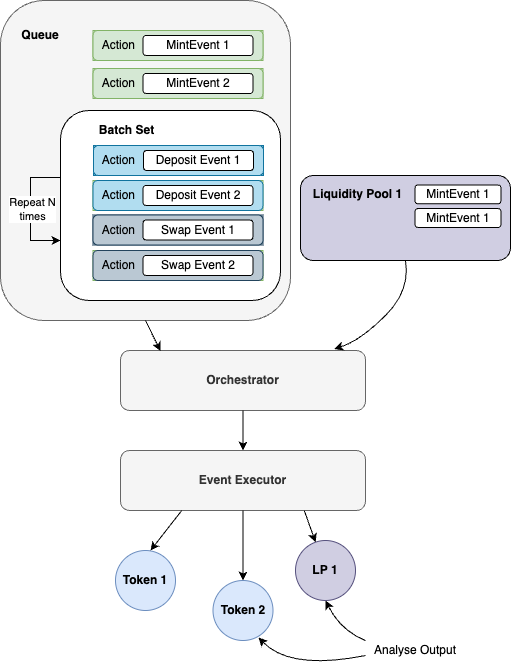
\includegraphics[width=3in]{img/simulator.png}
\caption{System components to DeFi Python simulator for DAOSYS} 
\label{fig:simulator}
\end{figure} 

\section{RoadMap}
\label{sec:roadmap}

\subsection{SYS Labs}

SYS Labs is the R\&D development arm of the Syscoin Platform which is to be self-perpetually funded through DAOSYS, hence being its own bank. It will do this by lending its earned funds to build the ecosystem, and increasing inherent value in a virtuous cycle of utility. We understand that specific business models may become irrelevant over time as companies organically typically grow and die over time based on the inability to adapt its business practices and revenue models to the existing market trends, however the DAO model we have created is agnostic of revenue models and is completely driven by decentralized principles and tokenomics which are flexible to build value in the best way possible, maximizing the value of entire ecosystem with the minimal social and financial overhead costs. All of our products will be based on user acquisition, open source and extracting maximal value into the appreciation of the ecosystem.

\subsection{Network Enhanced Virtual Machine}

In Dec 2021, Syscoin released the first stage of its Network Enhanced Virtual Machine (NEVM) which utilizes the Ethereum Virtual Machine (EVM). In the coming months (from the time of this publication), this will include a Zero Knowledge Proof (ZKP) system to build layer 2 (L2) scalable applications \cite{Sig21a,Sig21b}, and one of the first of these applications will be DAOSYS.

\subsection{Usecases}

\subsubsection{Masternode Yield Farming}
\label{sec:yield_farming}

Yield farming is a technique that uses DeFi to maximize returns where investors submit liquidity to a decentralized application (ie, dApp) to earn yield on their principle using various methods. These methods are classified into four main types which include: staking, lending, borrowing, and utilizing liquidity providers, which is largely done on a decentralized exchange (DEX). 

Syscoin plans to incentivize Masternode operators where they can put yields to work by investing them into a DeFi liquidity provider which will be automated in a trustless manner through DAOSYS. Hence, extending the Syscoin ecosystem, and increasing daily volumes. This system of trustlessly investing Masternode yields into a DeFi liquidity provider is what we call \textit{Masternode Yield Farming}, which will serve as the first intended usecase for DAOSYS and will be the first of its kind in the crypto space.

Currently, there are approximately 2,500 Masternodes running on the Syscoin network. In \cite{Moo22A}, we ran a case study with a five-year projection analysis on an additional 400 Masternodes, while at the same time factoring in network growth. We applied all these components into our model to estimate daily supply growth of the network, along with its respective confidence intervals; see Appendix \ref{sec:masternode_tokenomics} for details. Overall, we are predicting an overall return of 14.7M SYS which represents a five-year return of 36.8\% from the original investment of 40M SYS; see Fig. \ref{fig:reward_output}. Without DAOSYS, we would only realize an overall return of 31.2\%. Keep in mind that the principle investment of 100K SYS is not subject to risk as the estimated DAOSYS returns are utilizing Masternode returns as its principle. With this tokenomics model, we estimated the expected share a typical node contributes to the network on a daily basis. Finally, with expected share, we estimated the five-year output of 400 new Masternodes; see Table \ref{table:mn_returns} for details.

\begin{figure}[h!]
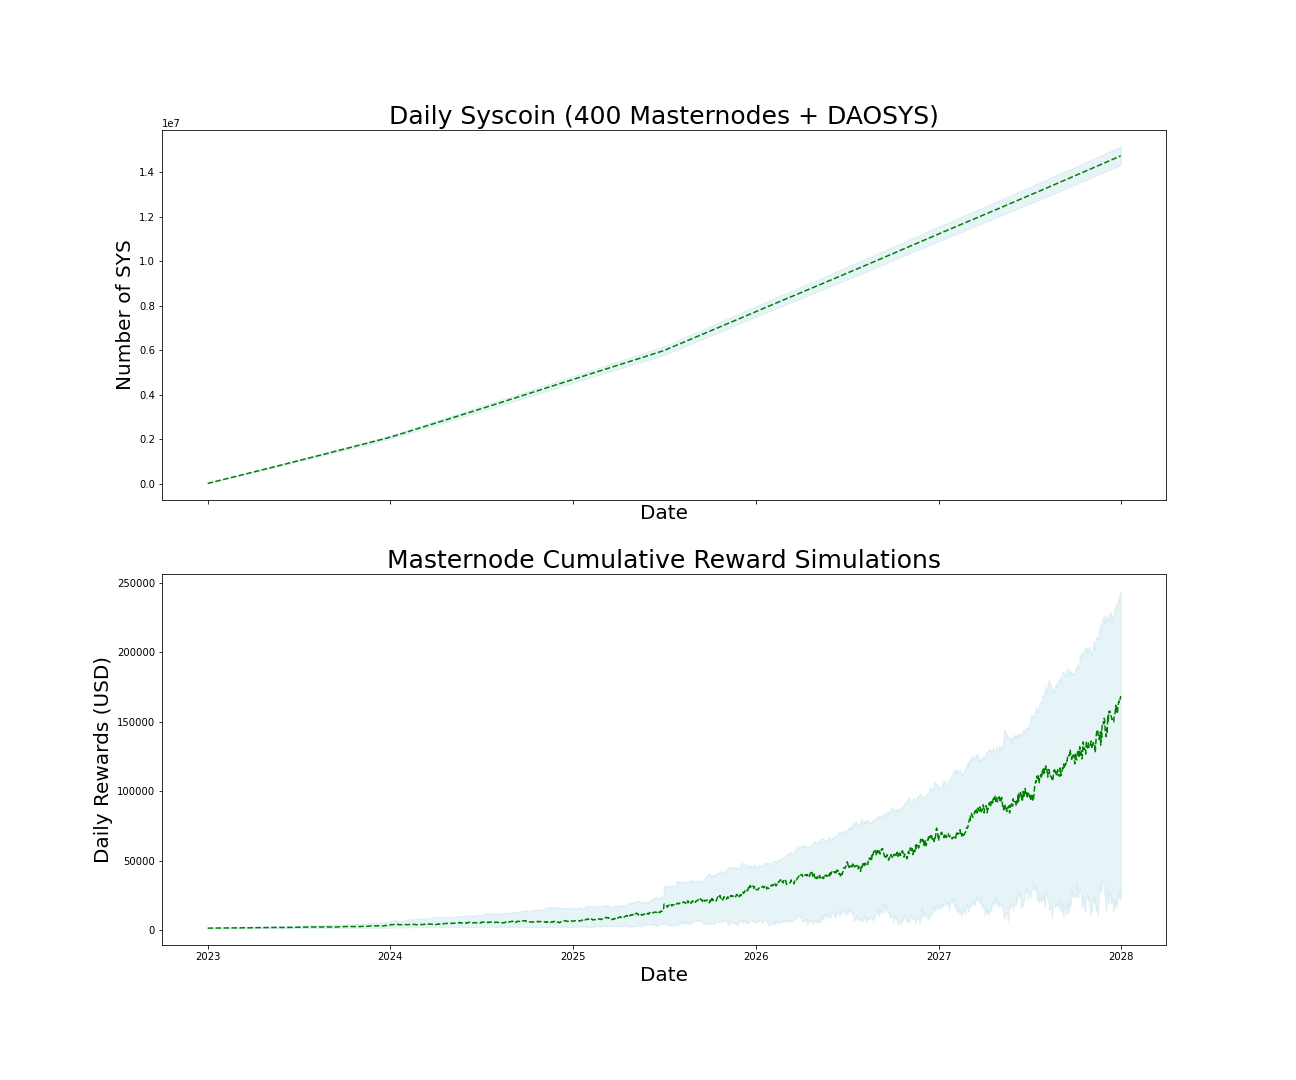
\includegraphics[width=3in]{img/supply_tot_reward_output.png}
\caption{Predicted five-year returns from 400 new Syscoin masternodes starting Jan 2023, which include both net positive yields from both Masternode and DAOSYS; (TOP) daily returns; and (BOTTOM) cumulative returns.} 
\label{fig:reward_output}
\end{figure} 

\begin{table}[h]
\centering
\begin{tabular}{ |c|c|c|c|c|c| } 
\hline
 \textbf{Date} & \textbf{USD} & \textbf{USD (lwr)} & \textbf{USD (upr)} & \textbf{nodes} \\
\hline
Dec 2023 & \$78,091 & \$51,283 & \$165,790 & 400 / 3,044\\
Dec 2024 & \$250,676 & \$75,868 & \$464,996  & 400 / 3,123 \\
Dec 2025 & \$931,645 & \$214,990 & \$1,540,776 & 400 / 3,198 \\
Dec 2026 & \$2,408,252 & \$534,067 & \$3,324,955 & 400 / 3,270 \\
Dec 2027 & \$5,246,669 & \$733,818 & \$7,265,095 & 400 / 3,338 \\
\hline
\end{tabular}
\caption{Projected monthly rewards from 400 investment nodes in USD using projected total (ie, Masternode + DAO SYS) rewards and Monte Carlo price simulations; see Appendix B}
\label{table:mn_returns}
\end{table}

The Syscoin Foundation will allocate \$20M SYS into SYS Labs. At an estimated \$27M USD peak valuation for 2023, SYS Labs will execute the master node yield strategy using its rewards. This will enable liquidity events which investors of SYS Labs can execute on through token warrants in exchange for equity. Masternode ROI will be used to deposit into DAOSYS which will be used to fund ecosystem initiatives as well as pay out token warrants to SYS Labs investors looking to exit. Analysis on Masternode ROI based on price modelling through to year 2028; see \cite{DAOSim22} for Jupyter notebook. Analysis on DAOSYS ROI based on price modelling through to year 2025 (not including value created through lending to builders to build ecosystem objectives); see \cite{DAOSim22}.

The same yield strategy (executed through DAOSYS) will also be executed to any of our own tokens we create through DeFi cloning protocols or tokens we create through our innovations (e.g., rollup gas tokens, wallet token, Luxy, ZKCross, etc.) where applicable. Token warrants would be issued and executed on via DAOSYS using an exit mechanism similar to the Masternode Yield Strategy. Also, the act of using DAOSYS to create an exit vehicle helps the remaining investors in the strategy by creating liquidity events that promote the growth of the DAO itself as well as the ecosystem. This is a form of vesting that matures over time. Thus giving unlimited upside potential at the expense of time value while maximizing positive effect of liquidity events instead of being parasitic to the rest of the investors.

\subsubsection{Index Tokens (Crypto ETFs)}

While the concept of indexing in the equity market is well established, it is surprising to see that this principle has yet to be largely applied to the crypto market using smart contracts. Hence, since DAOSYS itself is a non-speculated asset backed index of cryptos, for the first time we introduce a new class of cryptos called index tokens or crypto ETFs. The intelligence of the DAOSYS protocol will allow for the seamless, secure deployment of these index tokens using one of its readily available templates addressing this important usecase.

To put into perspective, under John Boogle’s direction, Vanguard is credited with the creation of the first index fund which was made available to the individual investor \cite{Bog17}. This index fund was created in 1957, and was passively tied to the performance of the S\&P 500. Boogle is known as the founder of The Vanguard Group, which as of today (ie, Sept 2022), manages \$7 trillion in assets. When investing long-term, Boogle argues the most efficient way to invest, is to simply buy the market itself, and that over time when looking at funds as a whole, they as a collective always revert to the mean. He also argues that over time, actively managed funds underperform the market, no matter what the current performance is.

Given the high volatility in the crypto market, and the fact that projects are continually entering and exiting the top 100 or even top 10 projects at a much higher frequency, we propose to simplify this problem and limit our attention to the top two crypos being BTC and ETH, with the introduction of what we term Bithereum. In Fig. \ref{fig:crypto_index} we see the advantage of developing an index token using this simple and effective strategy as we compare Bitcoin performance against the performance of various weighting strategies with Ethereum. Also, from a point of reasoning, it makes good sense to create an index token with BTC and ETH for the following reasons:

\begin{itemize}
  \item ETH and BTC have been the top two projects by market cap for the past 5 years
  \item ETH is a good proxy for the altcoin market which perform better in bull markets, while BTC is a good proxy for crypto gold which perform better in bear markets
  \item The combined market cap share of the crypto space of both of these two projects has fluctuated between 60-90\%
  \item Market cap share between ETH and BTC is negatively correlated against each other (p-val $\sim$ 0)
  \item ETH encapsulates large portions of other sectors (DeFi, NFT, etc) of the crypto space
\end{itemize}  

\begin{figure}[h!]
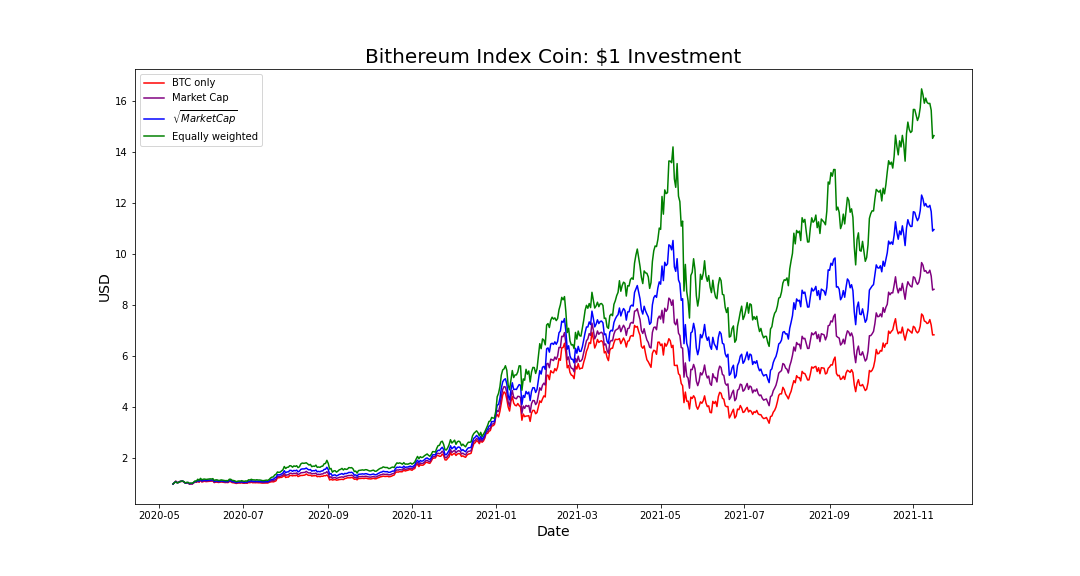
\includegraphics[width=3in]{img/index_coin.png}
\caption{Comparison of various Bithereum index coin market weighting strategies beginning at the 2020 BTC halvening with \$1 initial investment. We see that compared to just BTC alone, that a 50/50 weighting of BTC and ETH would outperform BTC by approximately 16 times.} 
\label{fig:crypto_index}
\end{figure} 

It is surprising that with all the developments that have happened in crypto, and given the success that ETFs have had in traditional finance, we have not yet seen adoption of this idea into crypto yet. However, DAOSYS with its smart DAO features will allow for the secure and seamless deployment of these new class of cryptos.  

\subsection{Launch Expectations}

Prior to mainnnet release, Syscoin's L2 (ie, Rollux) \cite{ROL22, Sig21a, Sig21b} must launch first along with Syscoin's Proof-of-Data Availability (PoDA) \cite{PODA22}. While it is technically possible that DAOSYS can run from any layer 1 (L1) EVM blockchain, it is our intention that it be launched when Rollux goes live. Currently, DAOSYS is running on the Rollux testnet where it is also running a test DAO for Pegasys, which is Syscoin's premiere decentralized exchange (DEX). 

We are expecting to launch DAOSYS in the early part of 2023 with crypto's first Masternode Yield Farm as its first functioning child DAO; see Fig. \ref{fig:daosys_launch}. Hence other projects running Masternodes will be incentivized to use our template and join the ecosystem to earn additional yield following the business case outlined in Section \ref{sec:yield_farming}.

\begin{figure}[h!]
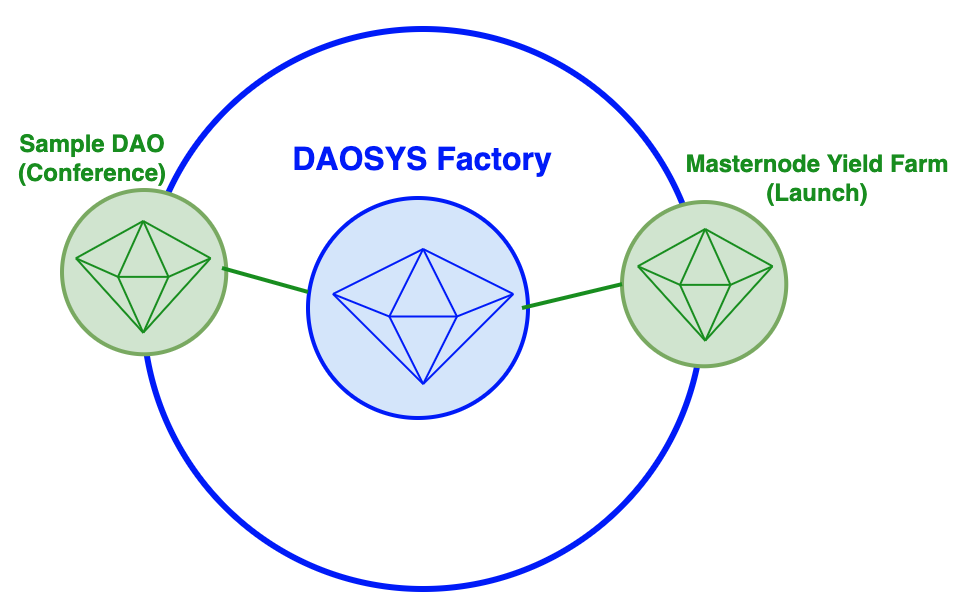
\includegraphics[width=3in]{img/daosys_launch.png}
\caption{DAOSYS expected ecosystem at launch in early 2023} 
\label{fig:daosys_launch}
\end{figure} 

\section{Summary}
\label{section:summary}

In this discussion we present the first ever smart DAO protocol; this idea is similar to Ethereum in the sense that both protocols work with decentralized immutable storage. However, instead launching contracts from chains, we work with Diamonds by exploiting the multi-facet proxy that was first presented in EIP-2535 \cite{Mud20}. To make the analogy, if Ethereum is the UNIX platform, then DAOSYS is the enterprise development system, which is utilized via low code or no code deployments.

DAOSYS allows for the self-sovereign capital coordination within decentralized organizations, which is the main problem that this project addresses. It does this via its new ASE technology which is made possible through an extension of the multi-facet proxy (ie, Diamonds) outlined in EIP-2535. We call this extension the Hyper-diamond standard.

DAOSYS is planning to launch on Rollux's mainnet in the early part of 2023, which is Syscoin's L2. During this event, we are also planning to launch the first of a new class of DAOs called Masternode Yield Farming. In this discussion, we have presented five-year ROI estimates using our DeFi python simulator that can also be used by community members who may be interested in testing out various business cases for DAO DeFi strategies. 

\appendices

\section{EIP-2535 (Diamond Facets)}
\label{sec:diamond}

EIP-2535 was an Ethereum proposal launched in 2020 to allow for the creation of modular contract systems that can be extended after deployment \cite{Mud20}. To solve this problem, this new proposal introduced a concept known as Diamonds. A Diamond refers to a smart contract system where functionality and storage is split up into separate contracts, and is an extension of a proxy contract.

A proxy contract is the the immutable part a user interacts with which holds data. It contains a fallback function which will catch any function call and use \texttt{delegatecall} to forward it to a second logic contract. A \texttt{delegatecall} will execute a function defined in the called contract (logic), but within the context of the calling contract (proxy). Thus, we have our logic defined separately from our data. This allows users to change the logic contract without changing the immutable underlying data. 

There are several limitations to proxy contracts which include: (a) implementing minor upgrades; (b) 24kb max contract size limit; (c) can only create identical proxy instances using one logic contract; and (d) cannot have a modular permission system. Diamonds solve these issues by allowing for multiple logic contracts which talks to the original proxy contract via the \texttt{delegatecall}; for comparison between these two systems see Fig. \ref{fig:diamonds} .

\begin{figure}[h!]
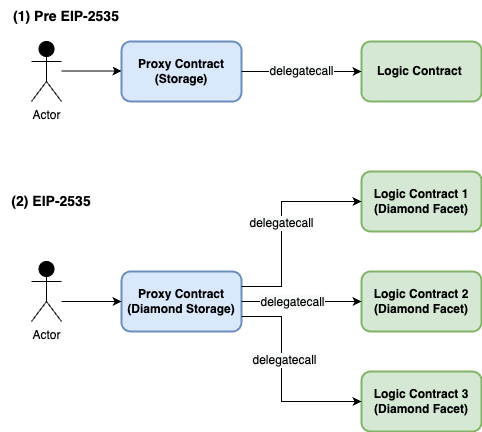
\includegraphics[width=3in]{img/diamonds.png}
\caption{Multi-facet proxy; (TOP) prior to EIP-2535, proxy contracts could only make delegates calls to another contract only; (BOTTOM) EIP-2535 introduced the capability of performing delegates calls to multiple contracts} 
\label{fig:diamonds}
\end{figure} 

\section{Masternode Tokenomics Model}
\label{sec:masternode_tokenomics}

The Masternode Yield Farming tokenomics model has two main components: (a) Masternode rewards; and (b) DAOSYS rewards. To acquire Masternode rewards, users stake liquidity to purchase a Masternode, thus used to generate $Coins_{New}$ in accordance to the specifications described in \cite{Sig21b}, which are as follows:

\begin{itemize}
\item \textbf{Block time:} 150 seconds
\item \textbf{Halving interval:} 210240 (1 year)
\item \textbf{Base Rewards:}  96.25 SYS per block deflated 5 percent every 210240 blocks
\item \textbf{NEVM Rewards:}  10.55 SYS per block (not deflated). EIP1559 model
\item \textbf{Governance Proposals:}  10 percent of Base Rewards paid out every 17520 blocks (1 month)
\item \textbf{Miner/Masternode Subsidy:}  90 percent of Base Rewards. 25 percent of this value goes to miner, 75 percent of this value goes to Masternode
\item \textbf{Masternode Minimum Subsidy:} 5.275 SYS (can not go below this amount even accounting for deflation)
\item \textbf{Masternode collateral requirement:} 100,000 SYS
\item \textbf{Masternode seniority}: 35 percent increase after 210240 blocks (1 year), 100 percent increase after 525600 blocks (2.5 years)
\end{itemize}
Using the rule set described above, we determine Masternode rewards via the following: 
\begin{equation*}
MN_{Rewards} = (Blocks_{Num}) (Coins_{New}) \left(\frac{Nodes_{Num}}{Supply_{Cur}}\right),
\end{equation*}
where current supply is calculated via the following:
\begin{equation*}
Supply_{Cur} = Supply_{Prev} + Coins_{New} - Fee_{TXBurn},
\end{equation*}
and $Fee_{TXBurn}$ is calculated in accordance to Section \ref{appendix:tx_fee_burn}. Finally, total rewards were determined via the following: 
\begin{equation*}
Total_{Rewards} = MN_{Rewards} + DAOSYS_{Rewards}. 
\end{equation*}
To estimate $DAOSYS_{Rewards}$, we used our DeFi python simulator; for tutorials and example templates one can reference \cite{Moo22B}. To estimate returns in USD, we applied the Monte Carlo procedure to estimate future point predictions for the USD value of Syscoin, as per Section \ref{appendix:monte_carlo}.

\subsection{Transaction Fee Burn}
\label{appendix:tx_fee_burn}

To model transaction fee burn to determine the supply end we used Ethereum fee data to serve as a proxy. We have determined that transaction fees follow an exponential growth that can be modelled via the following log-log model:
\begin{equation}
ln(\hat{y_{t}}) = a + bln(x_{t}),
\end{equation}
where parameters $a$ and $b$ and its confidence intervals can be estimated using Ordinary Least Squares (OLS).

\subsection{Price Point Predictions: Monte Carlo}
\label{appendix:monte_carlo}
To generate point predictions for the price of Syscoin, we made some assumptions. Price was given the freedom to fluctuate between \$0.25 to \$25 USD / SYS over the five-year projection interval (ie, 2023-2028) while maintaining an overall upward logarithmic growth, which is a price behavior characteristic that can be attributed to most successful crypto projects. To do this we generated a set of Monte Carlo point predictions, $\mathbf{\hat{p}}_{t}$, using the following:

\begin{equation}
\label{eqn:trend}
	\mathbf{\hat{p}}_{t} = c + \mathbf{\tilde{z}}_{t}e^{k z_{t}},
\end{equation}
where random drift term $\mathbf{\tilde{z}}_{t}$ is normalized between the interval [$a_{lwr}$,$a_{upr}$] as given by:
\begin{equation}
\label{eqn:min_max}
	\mathbf{\tilde{z}}_{t}= \frac{\mathbf{z}_{t} - min(\mathbf{z}_{t})}{max(\mathbf{z}_{t}) - min(\mathbf{z}_{t})},
\end{equation}
and $\mathbf{z}_{t}$ is an ARIMA(1,1,1) process, given by:
\begin{equation}
\label{eqn:drift}
	\mathbf{z}_{t} = \gamma + \mathbf{z}_{t-1} + \phi_{1} \mathbf{z}_{t-1} - \phi_{1} \mathbf{z}_{t-2} +  \theta_{1} \mathbf{e}_{r-1} + \mathbf{e}_{t},
\end{equation}
where $\phi_{1}$ is the AR(1) coefficient, $\theta_{1}$ is the MA(1) coefficient, and $\mathbf{e}_{t} \sim N(0, \sigma^2)$. Once these sets were generated, we estimated the 5$^{th}$ and 95$^{th}$ percentiles to attain the 90\% prediction interval. For a table of these point predictions along with its corresponding confidence interval, see \cite{Moo22A}. 

\begin{thebibliography}{00}

\bibitem{San83} S.J. Grossman, O.D. Hart, \textit{An Analysis of the Principal-Agent Problem}, Econometrica, Volume 51, Issue 1 (Jan., 1983), 7-46.

\bibitem{Sie22} D. Siegel, \textit{Understanding The DAO Attack}, Coindesk, Aug. 2022. Accessed on: Sept 2022. [Online]. Available: https://www.coindesk.com/learn/2016/06/25/understanding-the-dao-attack/

\bibitem{Sys22} Syscoin Dev Team, \textit{DAOSYS Lite Paper}, Accessed on: Sept 2022.  [Online]. Available:  https://github.com/syscoin/daosys

\bibitem{Uni19} Uniswap Blog, \textit{A short history of Uniswap}, Sept. 2019. Accessed on: Sept 2022.  [Online]. Available:  https://uniswap.org/blog/uniswap-history

\bibitem{Mud20} N. Mudge, \textit{EIP-2535: Diamonds, Multi-Facet Proxy}, Aug. 2020. Accessed on: Sept 2022.  [Online]. Available: https://eips.ethereum.org/EIPS/eip-2535

\bibitem{But18} V. Buterin, \textit{EIP-1014: Skinny CREATE2}, Apr. 2018. Accessed on: Sept 2022.  [Online]. Available: https://eips.ethereum.org/EIPS/eip-1014

\bibitem{Moo22A} I.C. Moore,  \textit{Masternode Yield Farming as a DAOSYS Usecase: Part 1}, Medium Article, Aug. 2022. Accessed on: Sept 2022.  [Online]. https://icmoore.medium.com/masternode-yield-farming-as-a-daosys-usecase-part-1-8485ab7ba721

\bibitem{Moo22B} I.C. Moore,  \textit{Masternode Yield Farming as a DAOSYS Usecase: Part 2}, Medium Article, Aug. 2022. Accessed on: Sept 2022.  [Online]. https://icmoore.medium.com/masternode-yield-farming-as-a-daosys-usecase-part-2-8906d0a11c27

\bibitem{DAOSim22} I.C. Moore, \textit{Simulation: Masternode Yield Farming}, Syscoin Github repos, Accessed on: Apr 2021.  [Online]. Available: https://github.com/syscoin/daosys/tree/main/notebooks/simulation

\bibitem{Bog17} J.C. Bogle, \textit{The Little Book of Common Sense Investing, 10th Edition}, John Wiley \& Sons, New Jersey, 2017

\bibitem{PODA22} Syscoin News, \textit{Syscoin PoDA is live on the Tanenbaum network!}, Syscoin, Aug. 2022. Accessed on: Sept 2022.  [Online]. Available: https://syscoin.org/news/syscoin-poda-is-live-on-the-tanenbaum-network

\bibitem{ROL22} Syscoin News, \textit{Introducing Rollux, Syscoin's Rollup Suite Ready to Take Market by Storm}, Syscoin, Jun. 2022. Accessed on: Sept 2022.  [Online]. Available: https://syscoin.org/news/introducing-rollux-syscoins-rollup-suite-ready-to-take-market-by-storm

\bibitem{Sig21a} J. Sidhu, \textit{A Design For An Efficient Coordinated Financial Computing Platform}, Feb 2021, Accessed on: Sep 2021.  [Online]. Available:  https://jsidhu.medium.com/a-design-for-an-efficient-coordinated-financial-computing-platform-ab27e8a825a0

\bibitem{Sig21b} J. Sidhu and I.C. Moore, \textit{Syscoin 4: A Peer-to-Peer Electronic Cash System Built For Decentralized
Web 3.0 Business Applications}, Syscoin Platform, Dec. 2021. Accessed on: Sept 2022. [Online]. Available: https://syscoin.org/$syscoin4\_whitepaper.pdf$



\end{thebibliography}


\EOD

\end{document}
